\section{Polarization properties of reflected light}

\begin{figure}[H]
    \centering
    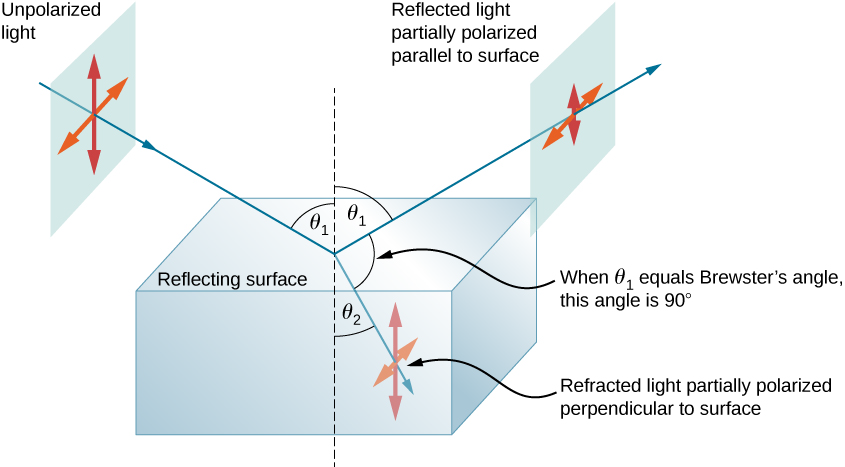
\includegraphics[width=\textwidth]{figures/polarization/reflaction.png}
    \caption{\blockquote{Polarization by reflection. Unpolarized light has equal amounts of vertical and horizontal polarization. After interaction with a surface, the vertical components are preferentially absorbed or refracted, leaving the reflected light more horizontally polarized. This is akin to arrows striking on their sides and bouncing off, whereas arrows striking on their tips go into the surface.}\cite[Figure 1.38]{lingUniversityPhysicsVolume2016}}
    \label{fig:polarized_reflection}
\end{figure}



\begin{align*}
    \centering
    r_\parallel = & \frac{\eta_1 \cos{\left(\theta_1 \right)} - \eta_2 \cos{\left(\theta_2 \right)}}
    {\eta_1 \cos{\left(\theta_1 \right)} + \eta_2 \cos{\left(\theta_2 \right)}}                        \\
    \\
    r_\perp     = & \frac{- \eta_1 \cos{\left(\theta_2 \right)} + \eta_2 \cos{\left(\theta_1 \right)}}
    {\eta_1 \cos{\left(\theta_2 \right)} + \eta_2 \cos{\left(\theta_1 \right)}}
\end{align*}

Where $r_\parallel$ and $r_\perp$ are the reflection coefficients for the lighe with a polarization parallel and perpendicular to the plane of incidence respectively.
$\eta_1$ is the refractive index of the air, $\eta_2$ is the refractive index of the water.
$\theta_i$ is the angle of incidence and $\theta_r$ is the angle of refraction.

Using the trigonometric identity $ \cos^2{\left(\theta_2 \right)} = 1- \sin^2{\left(\theta_2 \right)}$ and Snell's law $\eta_1 \sin{\left(\theta_1 \right)} = \eta_2 \sin{\left(\theta_2 \right)}$ the reflection coefficients angle of refrection can be removed and the equations can be written as:

\begin{align}
    r_\parallel = & \frac{\eta_1 \cos{\left(\theta_1 \right)} - \sqrt{- \eta_1^{2} \sin^{2}{\left(\theta_1 \right)} + \eta_2^{2}}}
    {\eta_1 \cos{\left(\theta_1 \right)} + \sqrt{- \eta_1^{2} \sin^{2}{\left(\theta_1 \right)} + \eta_2^{2}}}                                   \\
    \\
    r_\perp     = & \frac{- \eta_1 \sqrt{- \eta_1^{2} \sin^{2}{\left(\theta_1 \right)} + \eta_2^{2}} + \eta_2^{2} \cos{\left(\theta_1 \right)}}
    {\eta_1 \sqrt{- \eta_1^{2} \sin^{2}{\left(\theta_1 \right)} + \eta_2^{2}} + \eta_2^{2} \cos{\left(\theta_1 \right)}}
\end{align}


